\hrefsection{tsfi.ls.lan}{\tsfisectionname{ls.lan}}



\lslan{} is a logical interface to the IT products in the LAN, that is
accessible via the physical interface \intf{PS.LAN}. The interface comprises the
protocols listed in \tableref{tab:ls.lan.protocols-ports} together with their
port numbers. \figureref{fig:tsfi.ls.lan.protocols} depicts the protocols that
contribute to the security aspects of the TSFI (see also the introductory
remarks in \chapterref{tsfi.ls}.

\begin{description}
\item[Ethernet] for the data link layer,
\item[IP] for routing,	
\item[TCP und UDP] for transport,
\item[DHCP] for address assignment in the LAN (TOE as client),
\item[TLS] for securing the communications with other IT prodducts in the LAN.
\item[HTTP\_Mgmt] HTTP for access to the management interface.
\end{description}

\tableref{tab:ls.lan.protocols-ports} lists protocols and their ports in more
detail. Figure~\vref{fig:tsfi.ls.lan.protocols} shows the protocols of interface
\lslan{} in relation to each other and to the TCP/IP layer model.

\afterpage{%
  \clearpage% Flush earlier floats (otherwise order might not be correct)
  \begin{landscape}% Landscape page
    \centering % Center table
    {
      \label{tab:ls.lan.protocols-ports}
\begin{longtable}{@{}lcllcclp{6cm}@{}}
  \toprule
  Service & In/Out & Protocol & via & Source port & Dest. port & TSFI & Note \\ \midrule \endhead
  \bottomrule \caption*{Protocols und port numbers for IP/TCP/UDP on \formatintf{LS.LAN}} \endfoot
  \bottomrule \caption{Protocols und port numbers for IP/TCP/UDP on \formatintf{LS.LAN}} \endlastfoot
  Base protocols & -- & IEEE802.3 &  -- & -- & -- &    \tsfilink{ls.lan.ether} \\
  & -- & IPv4 & IEEE802.3 & -- & -- &    \tsfilink{ls.lan.ip} \\
  & -- & TCP &  IPv4 & -- & -- &    \tsfilink{ls.lan.tcp} \\
  & -- & UDP &  IPv4 & -- & -- &    \tsfilink{ls.lan.udp} \\[2ex]
  Administration & In & TLS & TCP & any & 9443 & \tsfilink{ls.lan.tls} & \\ 
  & In & HTTP & TLS & any & 9443 &  \tsfilink{ls.lan.httpmgmt} \\[2ex]
\end{longtable}


%

%!TEX root = "../adv_fsp"
%%% Local Variables:
%%% mode: latex
%%% TeX-engine: luatex
%%% TeX-master: "../adv_fsp"
%%% TeX-parse-self: t
%%% TeX-auto-save: t
%%% End:

    }
  \end{landscape}
  \clearpage% Flush page
}

\begin{figure}[htbp]
  \centering
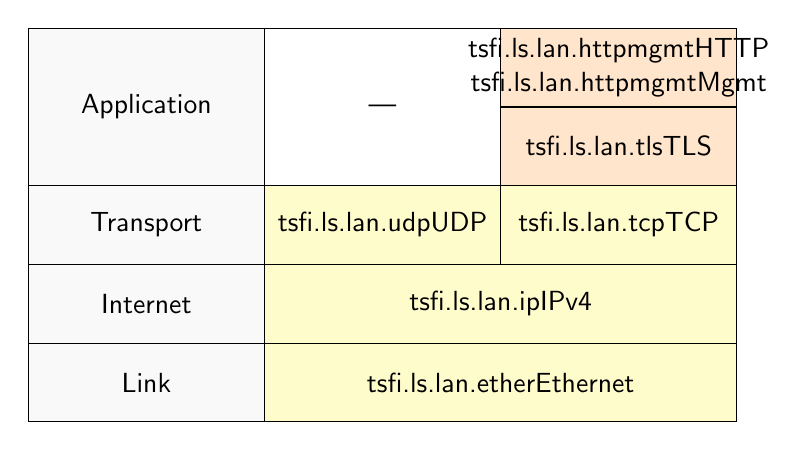
\begin{tikzpicture}
    [c/.style={midway,align=center,font=\sffamily},
      tsfi/.style={fill=orange!20},
      nontsfi/.style={fill=yellow!20},
      none/.style={},
      layer/.style={fill=gray!5}]


  % App Layer für UDP
  \draw[layer] (0,3) rectangle ++(3,2) node[c]{Application};
  \draw[none] (3,3) rectangle ++(3,2) node[c]{---};
  \draw[tsfi] (6,3) rectangle ++(3,1) node[c]{\hyperlink{tsfi.ls.lan.tls}{TLS}};

  \draw[tsfi] (6,4) rectangle ++(3,1) node[c]{\hyperlink{tsfi.ls.lan.httpmgmt}%
    {HTTP}\\\hyperlink{tsfi.ls.lan.httpmgmt}{Mgmt}};

  % Transport Layer
  \draw[layer] (0,2) rectangle ++(3,1) node[c]{Transport};
  \draw[nontsfi] (3,2) rectangle ++(3,1) node[c]{\hyperlink{tsfi.ls.lan.udp}{UDP}};
  \draw[nontsfi] (6,2) rectangle ++(3,1) node[c]{\hyperlink{tsfi.ls.lan.tcp}{TCP}};

  % IP Layer
  \draw[layer] (0,1) rectangle ++(3,1) node[c]{Internet};
  \draw[nontsfi] (3,1) rectangle ++(6,1) node[c]{\hyperlink{tsfi.ls.lan.ip}{IPv4}};

  % Network Layer
  \draw[layer] (0,0) rectangle ++(3,1) node[c]{Link};
  \draw[nontsfi] (3,0) rectangle ++(6,1) node[c]{\hyperlink{tsfi.ls.lan.ether}{Ethernet}};

\end{tikzpicture}
  \caption{Protocols on \formatintf{LS.LAN} for the TSFI}
  \label{fig:tsfi.ls.lan.protocols}
\end{figure}

\clearpage

\hrefsubsection{tsfi.ls.lan.ether}{\tsfisectionname{ls.lan.ether}}

\tsfipurpose{tsfi.ls.lan.ether}

This interface servers as the \emph{data link layer} to the ethernet network.

\calledsf{ls.lan.ether}

\tsfiparameters{tsfi.ls.lan.ether}

This interface implements the ethernet protocol as specified in
\autocite{IEEE802.3}.

\hrefsubsection{tsfi.ls.lan.ip}{\tsfisectionname{ls.lan.ip}}

\tsfipurpose{tsfi.ls.lan.ip}

This interface implements the \emph{internet layer}. On the internet layer, the
TOE supports IPv4. Additionally, the TOE supports ICMP (which is part of IP).

\calledsf{ls.lan.ip}

\tsfiparameters{tsfi.ls.lan.ip}

The implementation of IPv4 fulfills the requirements from \rfc[c]{791},
\rfc[c]{1812} and the update in \rfc[c]{2644}. ICMP is specified in
\rfc[c]{792}. The Linux kernel provides the protocol implementation.

\hrefsubsection{tsfi.ls.lan.tcp}{\tsfisectionname{ls.lan.tcp}}

\tsfipurpose{tsfi.ls.lan.tcp}

This interface implements the \emph{transport layer}. The TOE implements the
Transmission Control Protocol.

\calledsf{ls.lan.tcp}

\tsfiparameters{tsfi.ls.lan.tcp}

The implementation of TCP fulfills the requirements from \rfc[c]{793}. The Linux
kernel provides the protocol implementation.

\hrefsubsection{tsfi.ls.lan.udp}{\tsfisectionname{ls.lan.udp}}

\tsfipurpose{tsfi.ls.lan.udp}

This interface implements the \emph{transport layer}. The TOE implements the
User Datagram Protocol (UDP).

\calledsf{ls.lan.udp}

\tsfiparameters{tsfi.ls.lan.udp}

The implementation of UDP fulfills the requirements from \rfc[c]{768}. The Linux
kernel provides the protocol implementation.

\hrefsubsection{tsfi.ls.lan.tls}{\tsfisectionname{ls.lan.tls}}

\tsfipurpose{tsfi.ls.lan.tls}

\lslantls{} is used to secure the communications to other IP products in the
LAN. TLS provides confidentiality and integrity to the connections. An overview
of the TLS connections of the TOE in listed in \tableref{tab:tlsconnections}.

\calledsf{ls.lan.tls}

\tsfiparameters{tsfi.ls.lan.tls}

The implementation of TLS fulfills the requirements from \rfc[c]{5246}. The
description of the TLS implementation and all TLS connections of the TOE are
documented in \sectref{sf.tls}.

\hrefsubsection{tsfi.ls.lan.httpmgmt}{\tsfisectionname{ls.lan.httpmgmt}}

\tsfipurpose{tsfi.ls.lan.httpmgmt}

The TOE implements an HTTP server for communication with the management web
application. Confguration data is transported in JSON notation. The protocol is
defined as a REST API. Measures are taken to prevent XSS and CSRF attacks. This
is described in detail in the Security Architecture \autocite{adv_arc}.

\calledsf{ls.lan.httpmgmt}

\tsfiparameters{tsfi.ls.lan.httpmgmt}

The HTTP server implements \rfc[c]{2616}. The parameters of the REST API are
documented in the guidance documentation \autocite{agd_adm}. JSON is specified
in \rfc[c]{7159}.


% !TEX root = "../adv_fsp"
%%% Local Variables:
%%% mode: latex
%%% TeX-engine: luatex
%%% TeX-master: "../adv_fsp"
%%% TeX-parse-self: t
%%% TeX-auto-save: t
%%% End:
